\documentclass[crop,tikz]{standalone}
\usetikzlibrary{backgrounds}
\colorlet{blue}{cyan}
\tikzset{
  inverted/.style = {
    color=white,
    background rectangle/.style={fill},
    show background rectangle
  }
}

\usetikzlibrary{decorations.markings,patterns}

\tikzset{%
  >=latex, % default arrow style
  ->-/.style={postaction={decorate},decoration={%
      markings,mark=at position #1 with {\arrow{>}}%
    }%
  },%
  ->-/.default=.5,%
  -<-/.style={postaction={decorate},decoration={%
      markings,mark=at position #1 with {\arrowreversed{>}}%
    }%
  },%
  -<-/.default=.5%
}

% eye
\newcommand{\eye}[4]{% size, x, y, rotation
  \draw[rotate around={#4:(#2,#3)}] (#2,#3) -- ++(-.5*55:#1) (#2,#3) -- ++(.5*55:#1);
  \draw (#2,#3) ++(#4+55:.75*#1) arc (#4+55:#4-55:.75*#1);
  % iris
  \draw[fill=gray] (#2,#3) ++(#4+55/3:.75*#1) arc (#4+180-55:#4+180+55:.28*#1);
  % pupil, a filled arc 
  \draw[fill=white] (#2,#3) ++(#4+55/3:.75*#1) arc (#4+55/3:#4-55/3:.75*#1);
}

\begin{document}
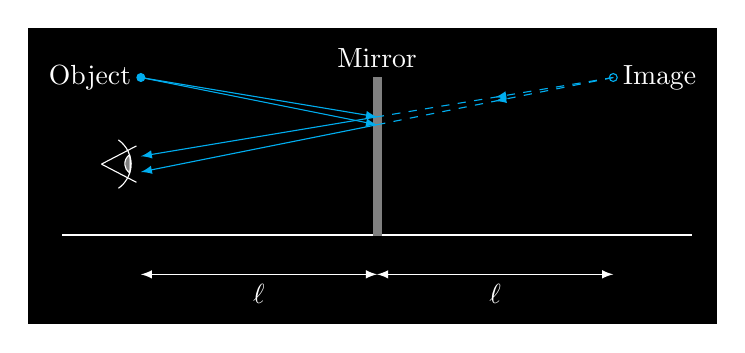
\begin{tikzpicture}[inverted,inverted]
  % floor
  \pattern[pattern=north east lines] (-4,0) -- ++(8,0) -- ++ (0,-0.2) -- ++(-8,0) -- cycle;
  \draw (-4,0) -- (4,0);
  % mirror
  \draw[fill,gray] (-0.05,0) rectangle (0.05,2);
  \node[above] at (0,2) {Mirror};
  % coordinates
  \pgfmathsetmacro{\xO}{-3};    % x coordinate of object
  \pgfmathsetmacro{\yO}{2};     % y coordinate of object
  \pgfmathsetmacro{\yOp}{1.5};  % 1st y coordinate on mirror
  \pgfmathsetmacro{\yOpp}{1.4}; % 2nd y coordinate on mirror
  \pgfmathsetmacro{\rO}{0.05};  % radius of object
  \coordinate (O) at ({\xO},{\yO});
  \coordinate (I) at ({-\xO},{\yO});
  \coordinate (M1) at (0,{\yOp});
  \coordinate (M2) at (0,{\yOpp});
  \coordinate (I1) at ({\xO},{\yO-2*(\yO-\yOp)});
  \coordinate (I2) at ({\xO},{\yO-2*(\yO-\yOpp)});
  % rays
  \draw[->,blue] (O) -- (M1);
  \draw[->,blue] (M1) -- (I1);
  \draw[->,blue] (O) -- (M2);
  \draw[->,blue] (M2) -- (I2);
  \draw[->-,blue,dashed] (I) -- (M1);
  \draw[->-,blue,dashed] (I) -- (M2);
  % points
  \draw[fill,blue] (O) circle ({\rO});
  \draw[blue] (I) circle ({\rO});
  % labels
  \node[left] at (O) {Object};
  \node[right] at (I) {Image};
  % eye
  \eye{0.5}{-3.5}{{-\yO+\yOp+\yOpp}}{0};
  % distance
  \draw[<->] (0,-0.5) -- node[below] {$\ell$} ++ ({\xO},0);
  \draw[<->] (0,-0.5) -- node[below] {$\ell$} ++ ({-\xO},0);
\end{tikzpicture}
\end{document}
